\documentclass{deltares_memo}
\svnid{$Id: plotcfts_um.tex 2031 2019-07-20 21:54:28Z mooiman $}
\svnid{$URL: file:///D:/SVNrepository/examples/plot_time_series_ugrid/trunk/doc/plotcfts_um.tex $}

\newcommand{\menuarrow}{$\rightarrow$}
\newcommand{\plotcfts}{PlotCFTS\xspace}
\newcommand{\qcustomplot}{QCustomPlot\xspace}
\newcommand{\netcdf}{NetCDF\xspace}
\newcommand{\cfstandard}{Climate and Forecast 1.7 standard\xspace}

\newcommand\T{\rule{0pt}{2.6ex}}       % Top T
\newcommand\B{\rule[-1.2ex]{0pt}{0pt}} % Bottom T
\begin{document}
\memoTo{To whom it may concern}
\memoConfidentialUntil{}
\memoDate{\today}
\memoVersion{001}
\memoFrom{Jan Mooiman}
\memoTelephone{+31\,(0)88\,335\,8568}
\memoEmail{jan.mooiman@deltares nl}
\memoSubject{Manual to plot \cfstandard compliant Time Series files}
\memoCopy{---}

\deltarestitle

%{{\footnotesize
%	{\textbf{Version control information}}
%	
%	\begin{tabular}{@{}p{12,5mm}@{}p{0mm}p{\textwidth-27mm-24pt}}
%		\textbf{Location} & \textbf{:} & \url{\svnkw{HeadURL}} \\
%		\textbf{Revision} & \textbf{:} & \svnrev 
%	\end{tabular}
%}}


\tableofcontents

%--------------------------------------------------------------------------------
\section{Release Notes}
\phantom{m}\vspace{-\baselineskip}
%
%--- begin light blue table ---
\begin{longtable}{p{16mm-12pt}|p{\textwidth-16mm-12pt}} 
%\caption{Light blue theme of table} \\% 
\rowcolor{dblue1} 
\textbf{Release} 
& \textbf{Description} 
\\ 
\topline 
\endfirsthead 
\endhead 
\endfoot 
\bottomline 
\endlastfoot 
2.09.00  &  - Some parameters where listed without having the time-dimension. Now a parameter need the time-dimension to be present in Parameter listbox.  \\
2.08.00  &  - Export to CSV, commas (,) in names replaced by semi-coumn (;).  \\
         &  - Fusion style theme used, advised by QT application. \\
2.07.00  &  - Show main window before loading the file given via the command line arguments.  \\
         &  - Time unit, now assigned once, so independent on the length of the time-series (a performance issue).  \\
2.06.00  &  - Disable reading a file with no time variable.  \\
2.05.00  &  - Export of \file{$\ast$.csv} file is now to start up directory.  \\    
2.04.00  &  - Location of selected graph added to the top of the context menu. \\
         &  - Double click on a selected graph shows the location, time and value of the point where the cursor is when the double click is performed.  \\
2.03.00  &  - Plot window is approximately a quarter of the main screen. \\
         &  - Main window size computed as percentage of the main screen. \\
         &  - Update spinners and tooltips if no files are in the file listbox.  \\
2.02.02  &  - Close option added to file menu, close will close the files and exit will exiting the program.  \\
2.02.01  &  - Set the tooltip to the filename which is selected in the file listbox.  \\
2.02.00  &  - Upgrade to QT 5.12.1.  \\
2.01.??  &  - No information available.  \\
\end{longtable} 
%--- end light blue table ---
%
%--------------------------------------------------------------------------------
\newpage
\section{Main window}
\phantom{m}\vspace{-\baselineskip}
\begin{figure}[H]
    \centering    
        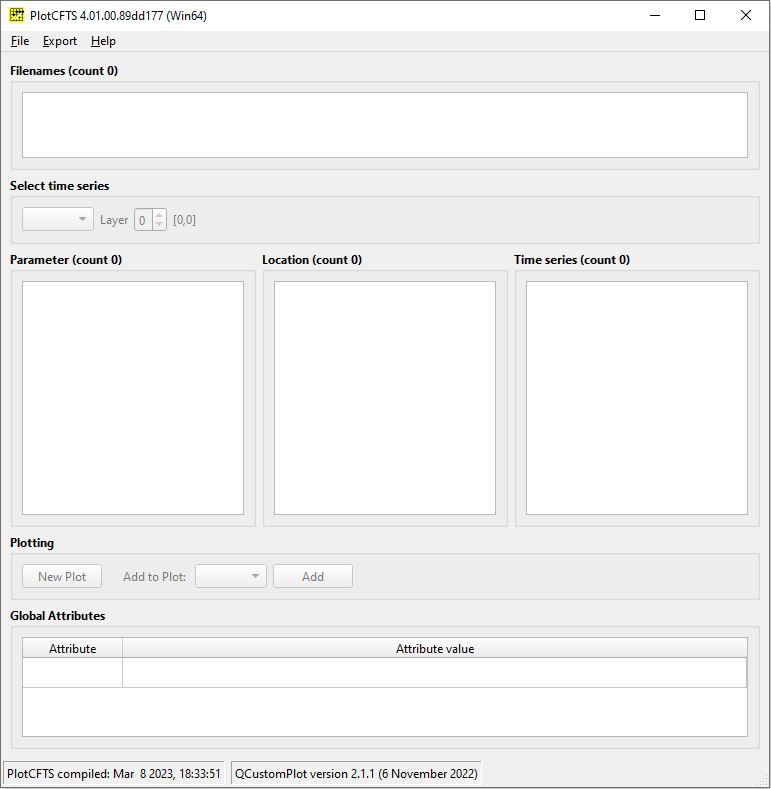
\includegraphics[width=0.9\textwidth]{pictures/main.png}
    \caption{Openings window of the program PlotCFTS (\textbf{Plot} \textbf{C}limate and \textbf{F}orecast \textbf{T}ime \textbf{S}eries)}
\end{figure}

%--------------------------------------------------------------------------------
\section{Menu bar}

%------------------------------------------------------------------------------
\subsection{File}
\phantom{m}\vspace{-\baselineskip}
\begin{figure}[H]
    \centering    
    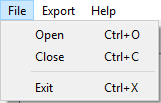
\includegraphics[width=0.20\textwidth]{pictures/menu_file.png}
    \caption{Menu \menuarrow File}
\end{figure}

%------------------------------------------------------------------------------
\subsubsection{Open file}
Open a file, all \netcdf files are shown, even if they do not met the \cfstandard.
If the file does met the Climate and Forecast standard 1.7 the file will be read and the main window will updated with the current information. 
%
\begin{figure}[H]
    \centering    
    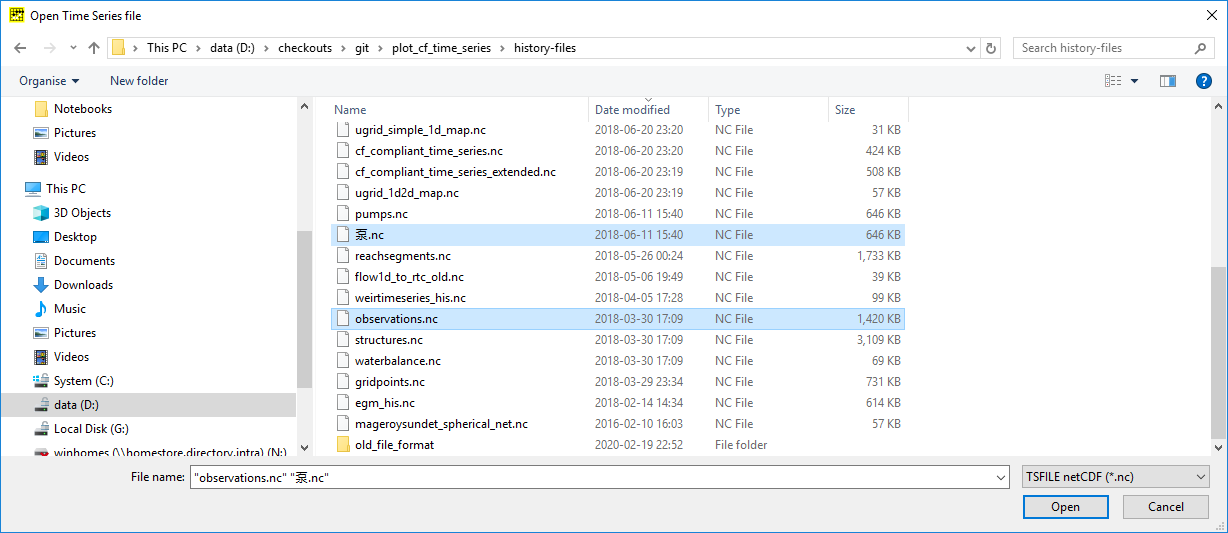
\includegraphics[width=0.9\textwidth]{pictures/menu_file_open.png}
    \caption{Open window, to open a \cfstandard compliant Time Series file (TSFILE)}
\end{figure}

If the file does not met the \cfstandard or cannot be read due to unsupported characters a message will presented (see \autoref{fig:notcffile})
\begin{figure}[H]
    \centering    
    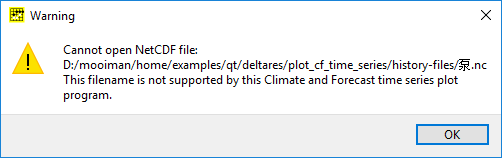
\includegraphics[width=0.6\textwidth]{pictures/message_not_cf_file.png}
    \caption{Message window when a file does not met the \cfstandard or the path contains unsupported characters.\label{fig:notcffile}}
\end{figure}

%------------------------------------------------------------------------------
\subsubsection{Close}
Close all plot windows and opened files.

%------------------------------------------------------------------------------
\subsubsection{Exit}
To exit the application \plotcfts.

%--------------------------------------------------------------------------------
\subsection{Export}
\phantom{m}\vspace{-\baselineskip}
\begin{figure}[H]
    \centering    
    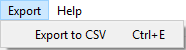
\includegraphics[width=0.20\textwidth]{pictures/menu_export.png}
    \caption{Menu \menuarrow Export}
\end{figure}

%------------------------------------------------------------------------------
\subsubsection{Export to CSV}
Export the data selected in the main program window to a comma separated value file. 
The default file name has as basename the current date/time combination  (ex.\ \file{2018-08-08\_230049}) and as extension \ext{csv}.
\begin{figure}[H]
    \centering    
    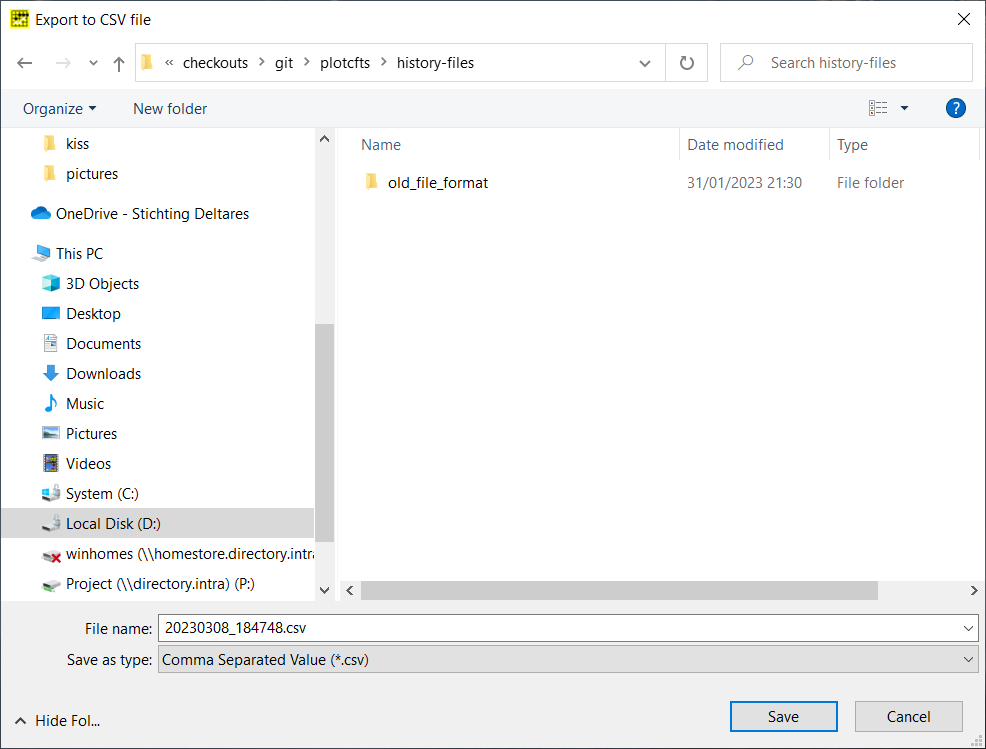
\includegraphics[width=0.9\textwidth]{pictures/menu_export_csv.png}
    \caption{Export window to export the data as indicated in the main window of the program \plotcfts.}
\end{figure}

%--------------------------------------------------------------------------------
\subsection{Help}
\phantom{m}\vspace{-\baselineskip}
\begin{figure}[H]
    \centering    
    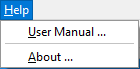
\includegraphics[width=0.2\textwidth]{pictures/menu_help.png}
    \caption{Menu \menuarrow Help}
\end{figure}

%--------------------------------------------------------------------------------
\subsubsection{User Manual}
Shows the user manual
\begin{figure}[H]
	\centering    
	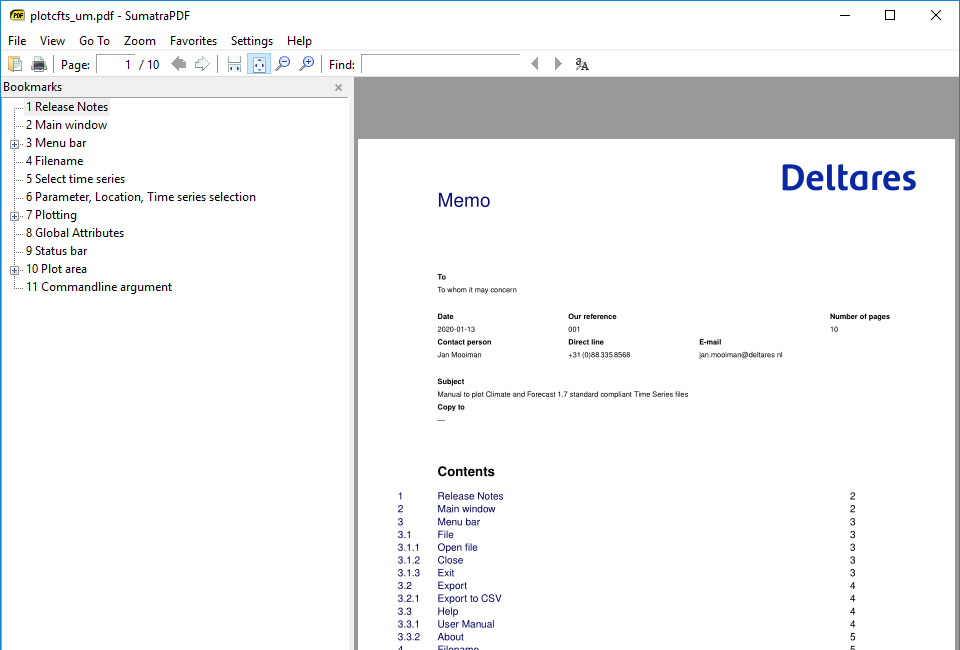
\includegraphics[width=0.9\textwidth]{pictures/menu_help_user_manual.png}
	\caption{PlotCFTS user manual}
\end{figure}

%--------------------------------------------------------------------------------
\subsubsection{About}
Shows the about box.
\begin{figure}[H]
    \centering    
    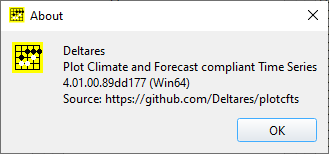
\includegraphics[width=0.4\textwidth]{pictures/menu_help_about.png}
    \caption{About box}
\end{figure}

%--------------------------------------------------------------------------------
\section{Filename}
\phantom{m}\vspace{-\baselineskip}
\begin{figure}[H]
    \centering    
    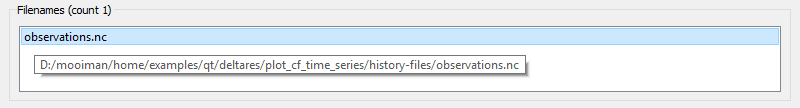
\includegraphics[width=0.9\textwidth]{pictures/group_filenames.png}
    \caption{List box for filenames.}
\end{figure}

%--------------------------------------------------------------------------------
\section{Select time series}
\phantom{m}\vspace{-\baselineskip}
\begin{figure}[H]
\centering    
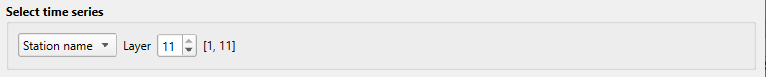
\includegraphics[width=0.9\textwidth]{pictures/group_select_time_series.png}
\caption{Combobox within group \menuarrow{Selected Time Series}}
\end{figure}

%--------------------------------------------------------------------------------
\section{Parameter, Location, Time series selection}
The groups \menu{Parameter, Location}  and \menu{Time series} are shown in \autoref{fig:groupplotting}:
\begin{figure}[H]
    \centering    
    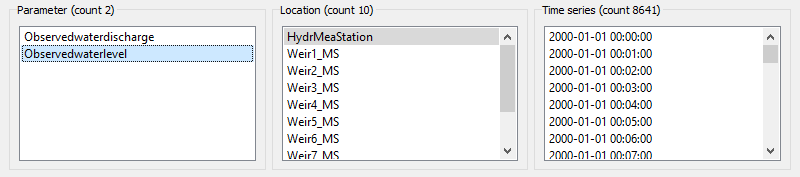
\includegraphics[width=0.9\textwidth]{pictures/group_parameter_location_time.png}
    \caption{List boxes for the Parameter, Location and Time Series.}
\end{figure}
With this group you are able to select a parameter(s) and a location(s) and the desired part of the time series. 
If no part of the time-series is selected thew whole time series will be used for plotting the graph.

%--------------------------------------------------------------------------------
\section{Plotting}
The group \menu{Plotting} is shown in \autoref{fig:groupplotting}:
\begin{figure}[H]
    \centering    
    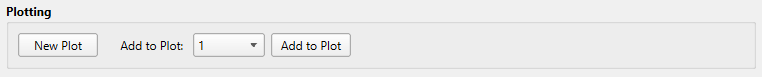
\includegraphics[width=0.9\textwidth]{pictures/group_plotting.png}
    \caption{Group Plotting. \label{fig:groupplotting}}
\end{figure}

%--------------------------------------------------------------------------------
\subsection{Button \button{New Plot}}
\phantom{m}\vspace{-\baselineskip}
\begin{figure}[H]
    \centering    
    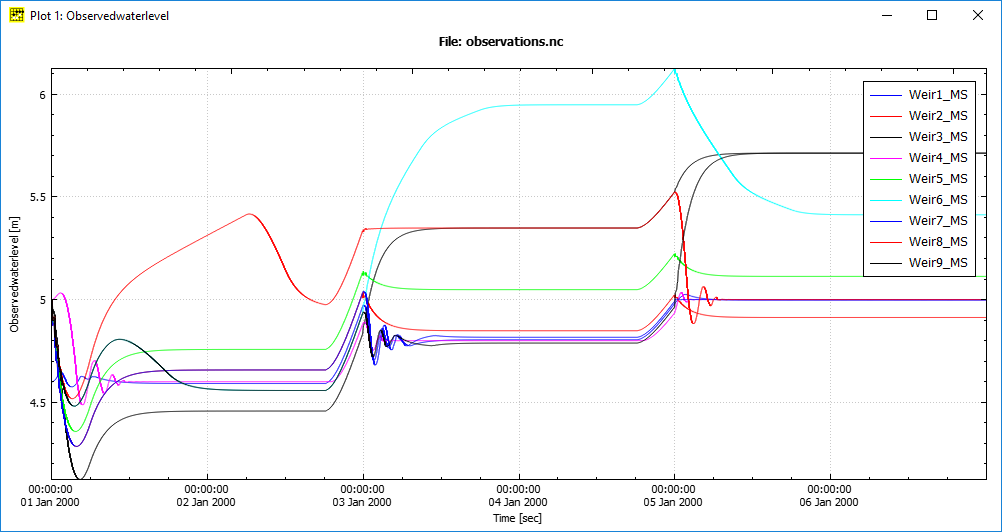
\includegraphics[width=0.9\textwidth]{pictures/plot.png}
    \caption{Initial plot after pressing button \emph{New Plot}}
\end{figure}
See \autoref{sec:howtohandleplot} for an explanation of available options to scale and rename some items of the plot area.
\subsection{Combobox next to button \button{Add}}
With this combobox you are able to select a plot by its number in which an additional graph can be plotted.

%--------------------------------------------------------------------------------
\subsection{Button \button{Add}}
When pressing this button the graph of the selected Parameter--Location will be added to the selected plot,idicated by the plot number.

%--------------------------------------------------------------------------------
\section{Global Attributes}
Showing the main global attributes as defined in the Climate and Forecast compliant Time Series file file (\netcdf format, see \autoref{fig:globalattributes}).
\begin{figure}[H]
    \centering    
    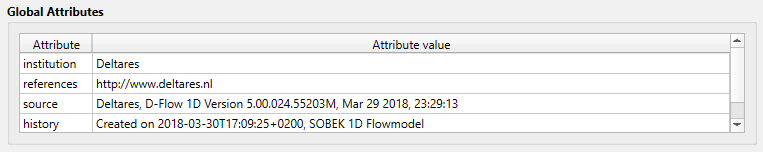
\includegraphics[width=0.9\textwidth]{pictures/group_global_attributes.png}
    \caption{Status bar\label{fig:globalattributes}}
\end{figure}

%--------------------------------------------------------------------------------
\section{Status bar}
The status bar present the compilation date and time, the version number of the used \qcustomplot library and the progress bar when reading a file (see \autoref{fig:statusbar}).
\begin{figure}[H]
    \centering    
    
\includegraphics[width=0.9\textwidth]{pictures/status_bar.png}
    \caption{Status bar\label{fig:statusbar}}
\end{figure}

%------------------------------------------------------------------------------
\section{Plot area\label{sec:howtohandleplot}}
\subsection{Zooming}
\phantom{m}\vspace{-\baselineskip}\begin{figure}[H]
    \centering
    \begin{subfigure}{0.3\textwidth}
    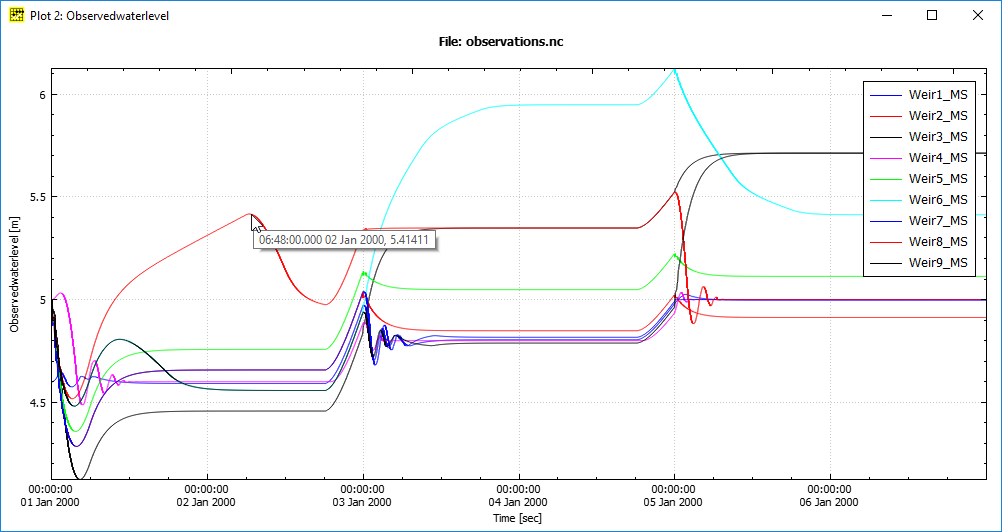
\includegraphics[width=\textwidth]{pictures/plot_zoom_point_multiplication.png}
    \caption{Point multiplication\newline}
    \end{subfigure}
\hfill
    \begin{subfigure}{0.3\textwidth}
    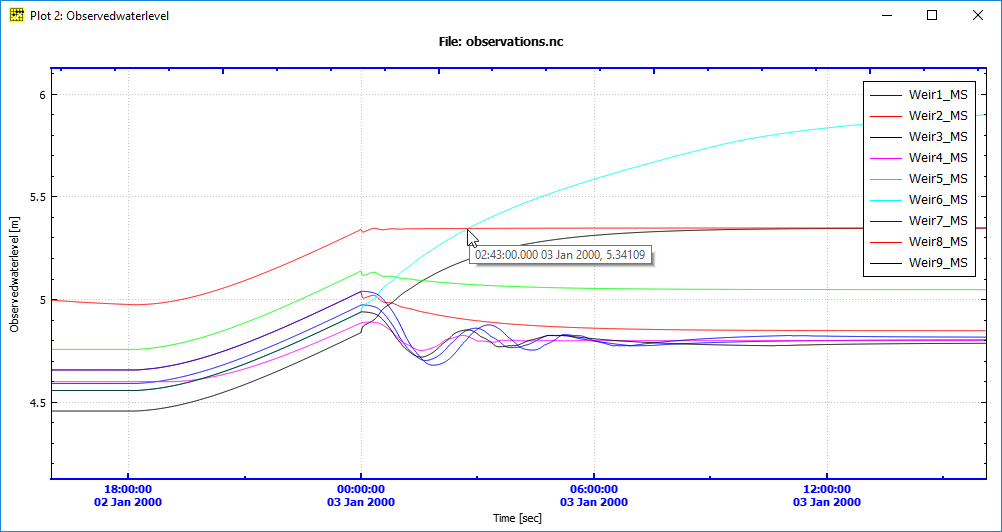
\includegraphics[width=\textwidth]{pictures/plot_zoom_x_axis.png}
    \caption{$x$-axis zooming, scaled by the scroll wheel}
    \end{subfigure}
\hfill
    \begin{subfigure}{0.3\textwidth}
    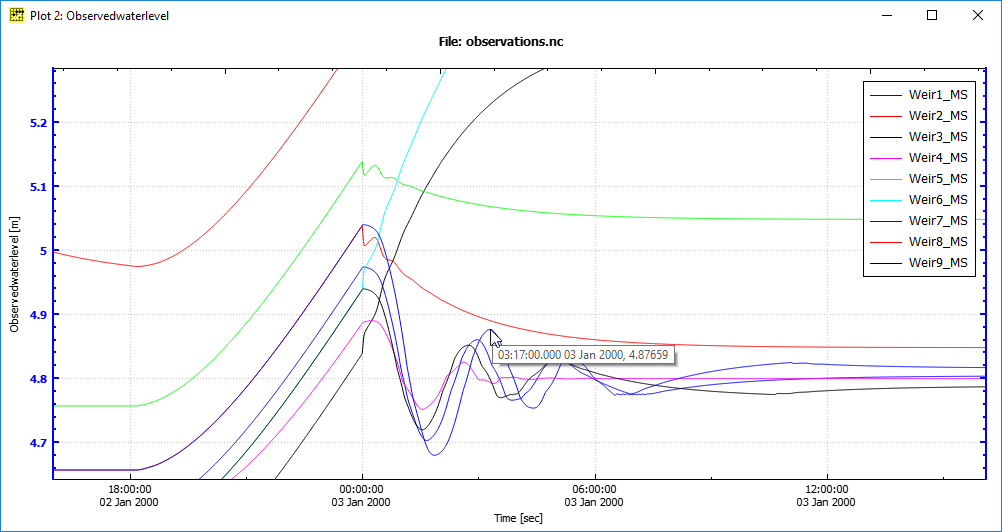
\includegraphics[width=\textwidth]{pictures/plot_zoom_y_axis.png}
    \caption{$y$-axis zooming, scaled by the scroll wheel}
\end{subfigure}
\caption{Several types of zooming: point multiplication, $x$-axis and $y$-axis. The zooming factor is scaled by the scroll wheel}
\end{figure}

%------------------------------------------------------------------------------
\subsection{Select a graph}
\phantom{m}\vspace{-\baselineskip}
\begin{figure}[H]
    \centering    
    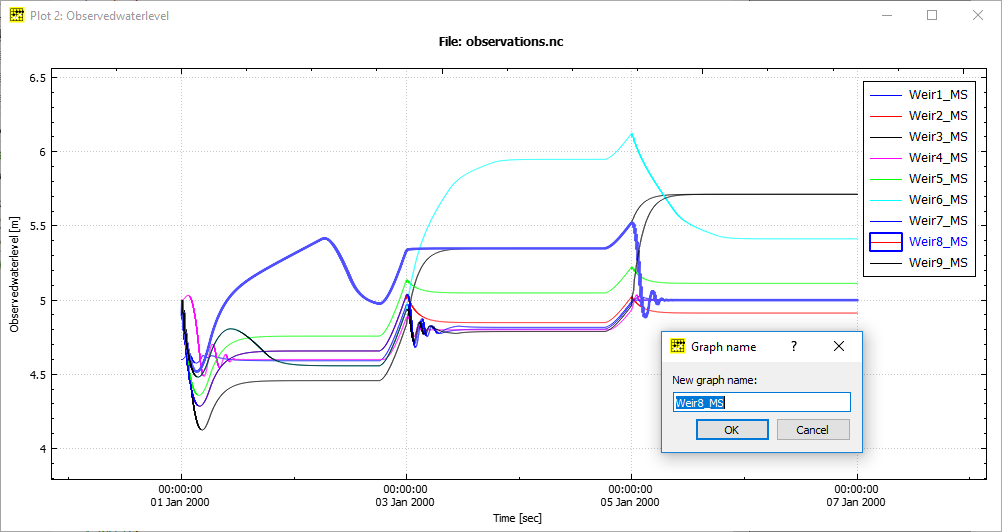
\includegraphics[width=0.9\textwidth]{pictures/plot_selected_graph.png}
    \caption{Graph selected and edit window for graph name\label{fig:selected graph}}
\end{figure}

%------------------------------------------------------------------------------
\subsection{Select a graph}
\phantom{m}\vspace{-\baselineskip}
\begin{figure}[H]
    \centering    
    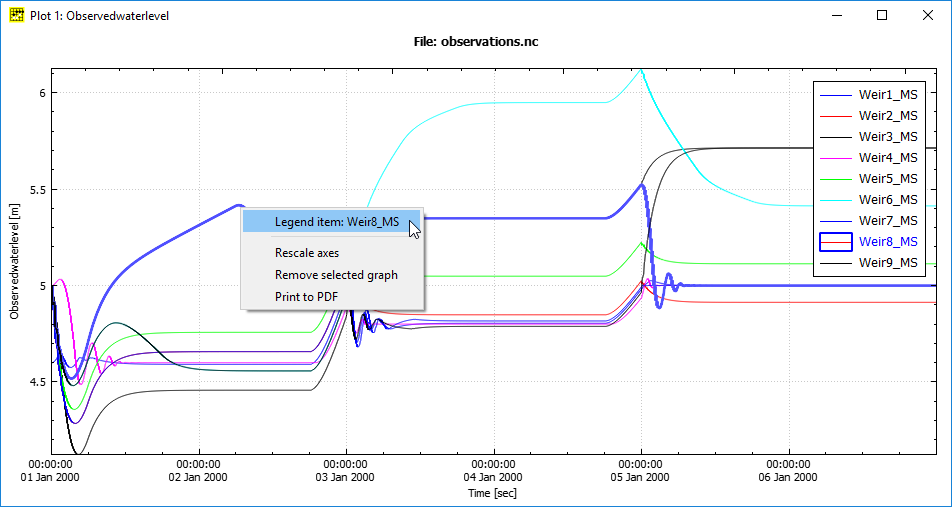
\includegraphics[width=0.9\textwidth]{pictures/plot_context_menu.png}
    \caption{Selected graph with context menu indicating the location in legend\label{fig:selected graph_with_context_menu}}
\end{figure}

%------------------------------------------------------------------------------
\subparagraph*{Context menu}
The context menu may have four items:
\begin{enumerate}
    \item \textbf{Legend item $\ast$:}\newline
    This item cannot be selected. 
    If a graph is selected the name of the location as presented in the legend is shown. 
    This context menu entry is useful when the plot area contains a lot of graphs and the legend area is too short.
    \item \textbf{Rescale axes}\newline
    Selecting this item the axes will be rescaled to the bounding box of the graphs.
    \item \textbf{Remove selected graph}\newline
    Selecting this item will remove the selected graph from the plot area and legend.
    \item \textbf{Print to PDF}\newline
    Selecting this item the plot will be saved to a pdf-file.
\end{enumerate}

%------------------------------------------------------------------------------
\subparagraph*{Double click on a selected graph}
When a double click is given on een selected graph a message window will shown the location, time and value of the point on the graph where the double click is performed.
\begin{figure}[H]
    \centering    
    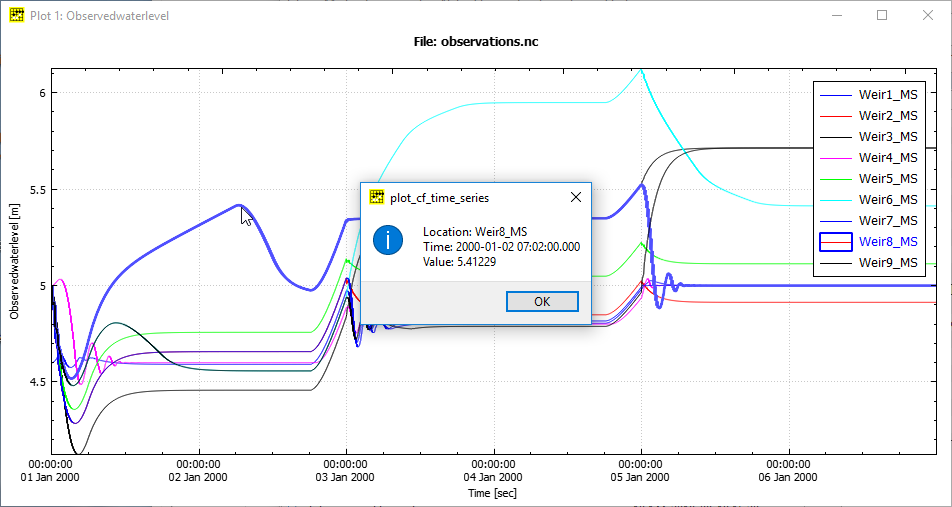
\includegraphics[width=0.9\textwidth]{pictures/plot_double_click_selected_graph.png}
    \caption{Selected graph with information window containing the location, time and value of the cursor location\label{fig:double_click_selected_graph}}
\end{figure}

%------------------------------------------------------------------------------
\subsection{Editing labels}

%------------------------------------------------------------------------------
\subsection{Multiple y-axis}
When multiple axis are needed each y-axis label gets a prefix, this label will also be visible as prefix in the legend.
\begin{figure}[H]
    \centering    
    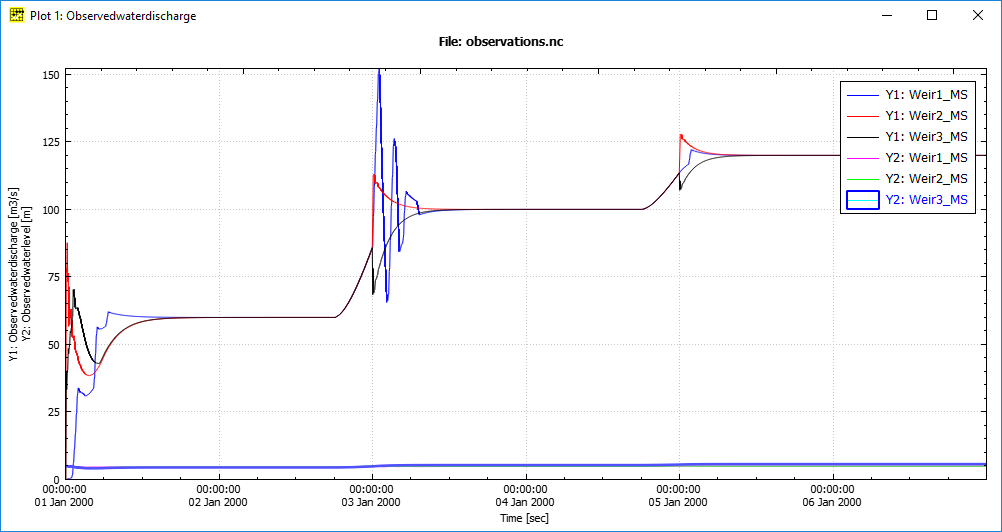
\includegraphics[width=0.9\textwidth]{pictures/multiple_yaxis.png}
    \caption{Multiple y-axis, legend and y-axis labels has a prefix. \label{fig:multiple y-axis}}
\end{figure}

%------------------------------------------------------------------------------
\subsection{Support ISO 10646 charaters set (UTF-8)}
The plot program support the ISO 10646 character set as seen in \autoref{fig:ChineseStation}, the location list box contains Norwegian and Chinese characters.
\begin{figure}[H]
    \centering    
    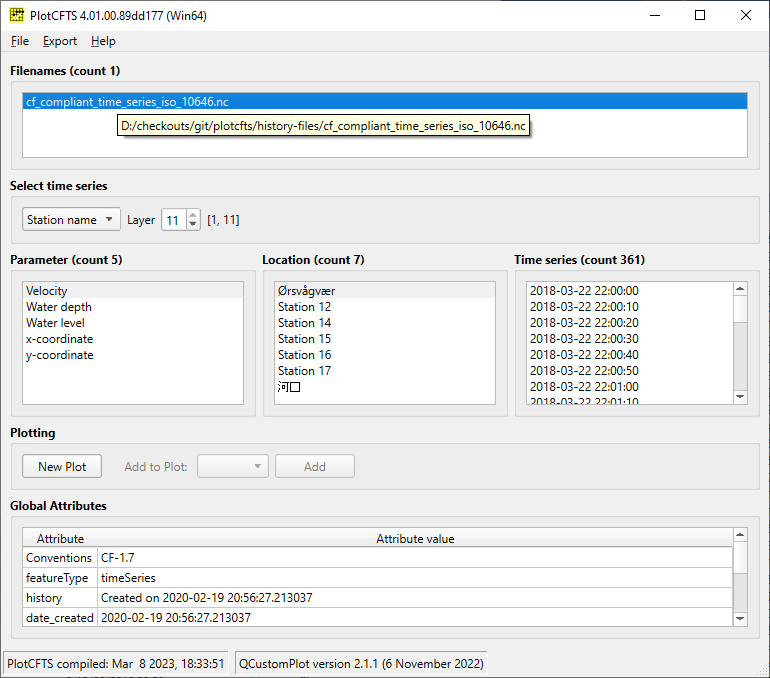
\includegraphics[width=0.9\textwidth]{pictures/plotcfts_with_chinese_karakters2.png}
    \caption{\emph{Location} list box contains Norwegian and Chinese characters. \label{fig:ChineseStation}}
\end{figure}

%------------------------------------------------------------------------------
\section{Commandline argument}
The program can be started with the desired file with a command line argument:
\begin{symbollist}
    \item[{-{}-ncfile}] Behind this argument the name of the NetCDF file need to be specified, including the file extension \ext{.nc}.
\end{symbollist}
\textbf{Example:}
\begin{Verbatim}
$ plocfts --ncfile <filename>
\end{Verbatim}

%------------------------------------------------------------------------------

\end{document}
